\chapter{Criptografia}
\label{cryptograhy}

%
A criptografia é a ciência dos códigos secretos, permitindo a confidencialidade de uma comunicação que utiliza um meio inseguro.~\cite{vauldenay}. Então a necessidade de manter informações em sigilo impulsionou a evolução dos estudos da criptografia. O exato início da criptografia é incerto, mas na Renascença,assim como outros em muitos outros campos, o estudo da criptografia começou a ser aprofundado e suas técnicas armazenadas e ensinadas. ~\cite{donald-davies}

%
Uma das primeiras formas de criptografia utilizada foi a substituição. A substituição primeiramente era feita de forma fixa, ou seja, era usada uma única tabela em que as letras do alfabeto eram trocadas por outras letras. Leon Battista Alberti introduziu uma maneira diferente de fazer a substituição, criando o algoritmo \textit{polyalphabetic substitution}. O princípio desse algoritmo era a criação de várias tabelas de substituição e a utilização de uma chave para definir a ordem que cada tabela seria usada para cifrar cada letra do texto em claro. O conjunto de tabelas de substituição é chamado de \textit{Vigenere tableau}.

%
Durante a II Guerra Mundial informações relacionadas a estratégias de guerra deveriam ser mantidas em sigilo. Com isso duas máquinas foram criadas e merecem destaque, a \textit{Enigma} e a \textit{SZ40}. Após a guerra, a publicação do algoritmo \textit{DES} serviu de incentivo para cientistas do mundo todo aprofundarem suas pesquisas em novos algoritmos. Nos dias de hoje existem duas linhas de estudo sobre a criptografia, a criptografia com chave simétrica e a com chave assimétrica. 

\begin{figure}[h]
\centering
\begin{minipage}{.5\textwidth}
  \centering
  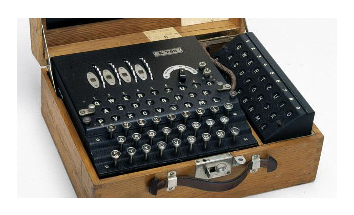
\includegraphics[keepaspectratio=true,scale=1]
  {figuras/enigma.eps}
  \caption{Máquina Enigma}
  \label{enigma-machine}
\end{minipage}%
\begin{minipage}{.5\textwidth}
  \centering
  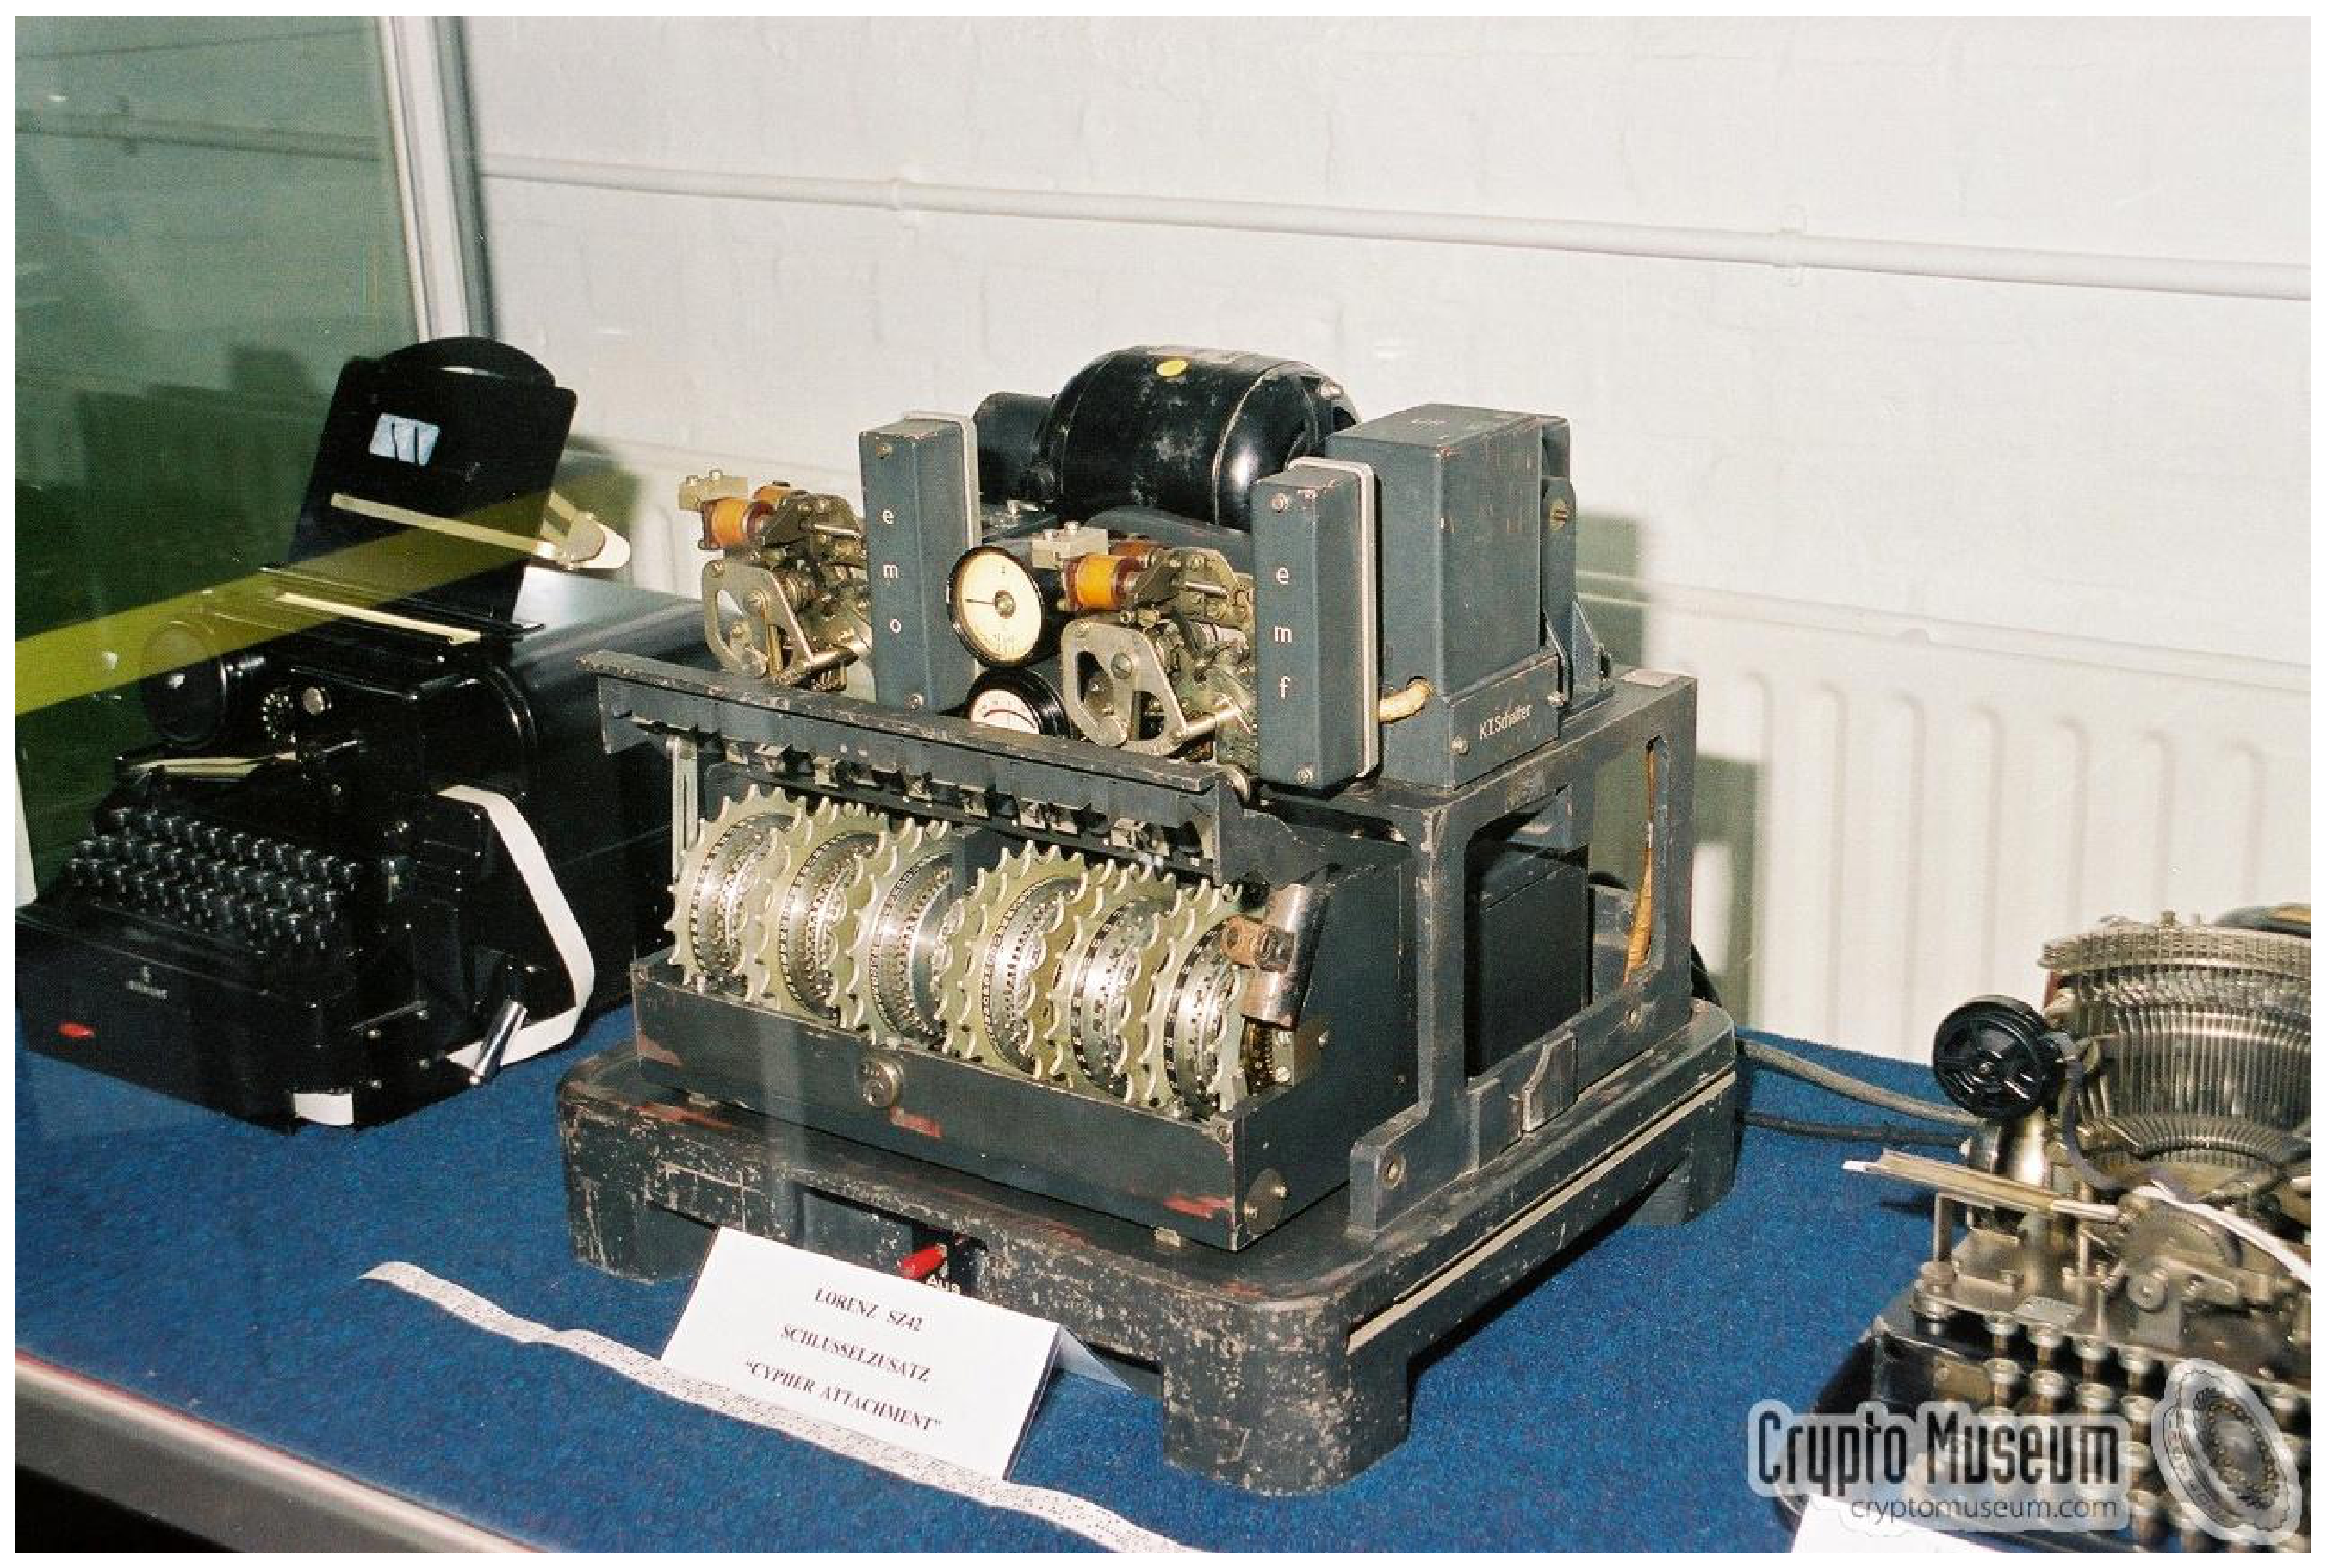
\includegraphics[keepaspectratio=true,scale=0.1]
  {figuras/sz40.eps}
  \caption{Máquina SZ40}
    \label{sz40-machine}
\end{minipage}
\end{figure}\footnote{ http://www.bbc.co.uk/history/topics/enigma e http://www.cryptomuseum.com/crypto/lorenz/sz40/}

%
\section{Termos}
\label{terms}

No decorrer do trabalho iremos utilizar alguns termos específicos do estudo da criptografia e essa seção visa apresenta-los e esclarece-los.

\begin{table}[h]
\begin{center}
    \begin{tabular}{|l| p{10cm}|}
    \hline
    Termo & Descrição \\ \hline
    Cifrar & Função que tem como objetivo transformar uma mensagem que deve estar em sigilo e transforma-la em algo inintelegível \\ \hline
    Decifrar & Função que transforma uma mensagem inintelegível para a mensagem original. \\ \hline
    Texto em claro & Mensagem que deve ser mantida em sigilo e que se deseja cifrar. \\ \hline
    Texto cifrado & Mensagem inintelegível e que se deseja decifrar. \\ \hline
    Chave & Entrada para as funções cifrar e decifrar, é usada para que duas pessoas consigam se comunicar em segredo. \\ \hline
    MDC & Operação matemática que visa descobrir o maior divisor comum entre dois ou mais números. \\ \hline
    $\phi$ & Teorema de Euler, retorna a quantidade de números inteiros positivos menores ou igual a um determinado número e que são primos relativos de desse número. \\ \hline 
    e & Chave pública, para cifrar um texto. \\ \hline
    d & Chave privada, para decrifrar um texto \\ \hline
    \end{tabular}
    \caption{Termos da criptografia}
\end{center}
\end{table}

%
\section{Criptografia Simétrica}
\label{symmetric-cryptography}

A criptografia simétrica utiliza a mesma chave para cifrar e decifrar uma mensagem. É objeto de estudo para muitos cientistas e existem muitos algoritmos que ainda são utilizados pelo mundo. Sua vantagem é que o custo para ser utilizada não é tão elevado e sua possibilidade de uso é maior. 

\begin{figure}[h]
\centering
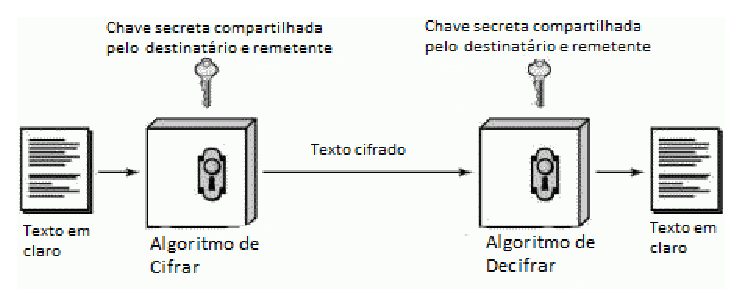
\includegraphics[scale=0.5]
{figuras/SymmetricCipher.eps}
\caption[Funcionamento básico da criptografia simétrica] {Funcionamento básico da criptografia simétrica\protect\footnotemark}
\end{figure}

\footnotetext{$http://www.codeproject.com/Articles/21076/Securing-Data-in-NET$}
Os algoritmos são divididos em: cifra de bloco e cifra de fluxo.

\subsection{Cifra de Bloco}
\label{block-cipher}

A cifra de bloco tem como princípio a cifra de blocos com tamanho definido e a mensagem criptografada deve ter o mesmo tamanho da mensagem em claro. Um algoritmo muito conhecido é o \textit{DES} e que foi desenvolvido pela \textit{IBM}. Foi a primeira cifra comercialmente desenvolvida e sua estrutura foi divulgada por completo. ~\cite{alex-biryukov}. 

O tamanho da chave utilizada no \textit{DES} é considerado um problema nos dias atuais. Muitos pesquisadores sabendo desse problema tentaram remediar o problema com novas maneiras criptográficas, um exemplo é o \textit{3-DES}, que utiliza duas chaves no processo, mas como consequência tem seu desempenho prejudicado. Outra medida para contornar o problema de ataques ao \textit{DES} foi a publicação de um concurso do \textit{NIST} para a escolha do novo padrão criptográfico. Assim surgiu o \textit{AES}, algoritmo que utiliza o sistema de permutação e substituição, tem o tamanho do bloco fixo de 128 bits e tamanho de chave variável entre 128, 192 ou 256 bits. 

Existem operações que podem ser aplicadas nas cifras de blocos e que podem ser utilizadas nos algoritmos \textit{DES} e \textit{AES} para a produção de mensagens criptografadas, são elas:

\begin{description}
\item [ECB]consiste em cifrar os blocos de forma independente um do outro e com uma chave fixa.
\begin{figure}[h]
\centering
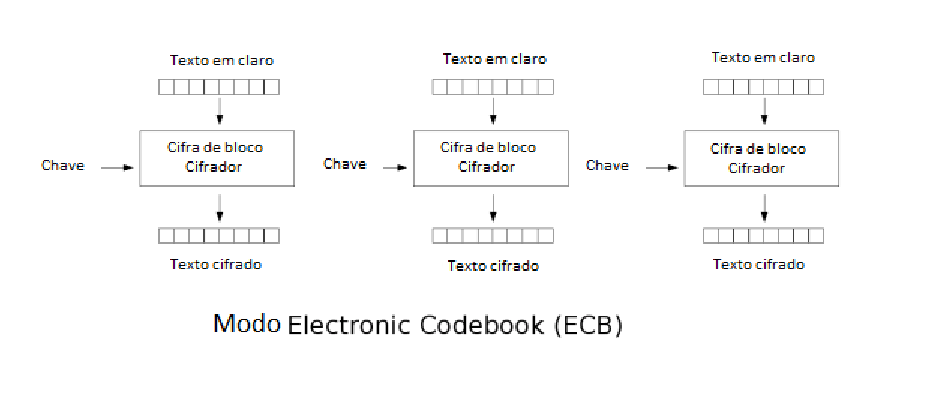
\includegraphics[keepaspectratio=true,scale=0.7]
	{figuras/ecb.eps}
	\caption{\textit{Electronic Codebook Mode}}
	
\end{figure} \footnote{$http://cryptodox.com/Block\_cipher\_modes\_of\_operation$}
\item[CBC] utiliza da operação de ou-exclusivo entre um vetor de inicialização( para o primeiro bloco) e o texto em claro e por fim um ou-exclusivo do resultado com a chave. A partir do segundo bloco ao invés de um vetor de inicialização é utilizado o bloco criptografado anterior.
\begin{figure}[h]
\centering
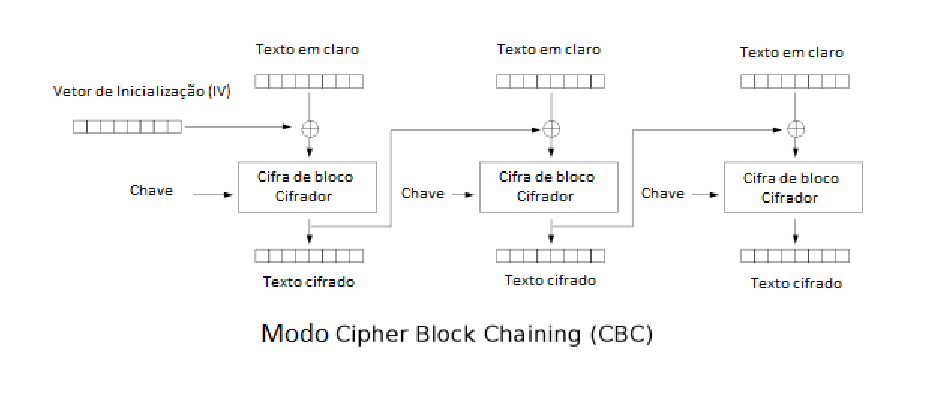
\includegraphics[keepaspectratio=true,scale=0.7]
    {figuras/cbc.eps}
    \caption{\textit{Cipher Block Chaining Mode}}
\end{figure} \footnote{$https://www.adayinthelifeof.nl/2010/12/08/encryption-operating-modes-ecb-vs-cbc/$}
\item[CFB] muito similar ao CBC, porém é feito um ou-exclusivo da chave com o vetor de inicialização ou bloco criptografado anterior e o resultado é feito um ou-exclusivo com a mensagem em claro.
\begin{figure}[h]
\centering
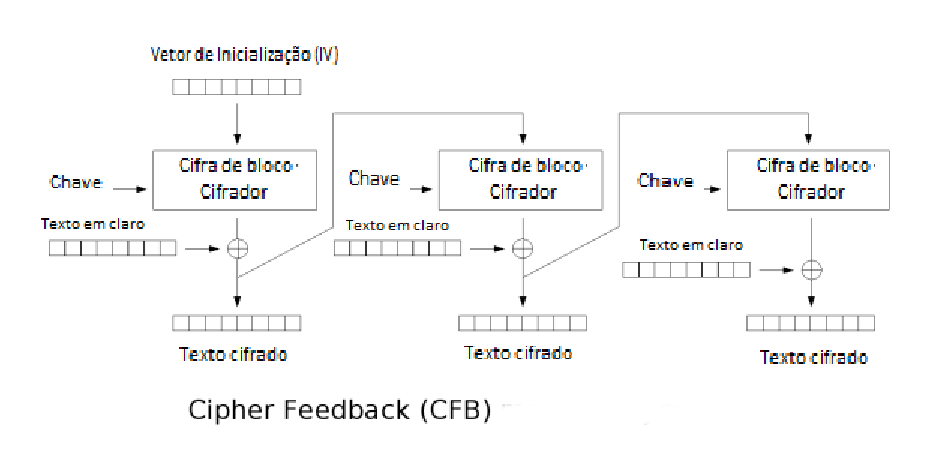
\includegraphics[keepaspectratio=true,scale=0.7]
    {figuras/cfb.eps}
    \caption{\textit{Cipher Feedback Mode } } 
\end{figure}\footnote{$http://crypto.stackexchange.com/questions/2476/cipher-feedback-mode$}
\item[OFB] a diferença em relação ao CFB é que o resultado entre o vetor de inicialização ou resultado da operação anterior e a chave serve de entrada para o próximo bloco, ao invés do bloco criptografado.
\begin{figure}[h]
\centering
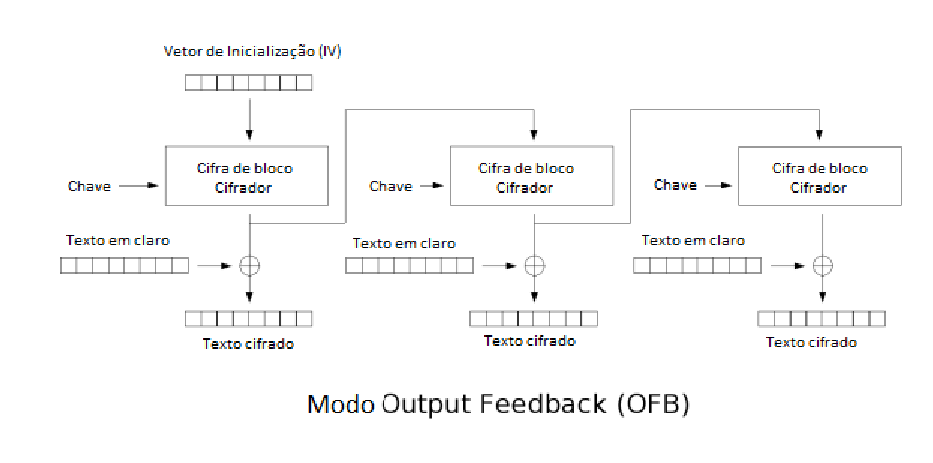
\includegraphics[keepaspectratio=true,scale=0.7]
    {figuras/ofb.eps}
    \caption{\textit{Output Feedback Mode } } 
\end{figure}\footnote{$http://commons.wikimedia.org/wiki/File:Ofb\_decryption.png$}
\item[CTR] utiliza como entrada para a função criptográfica um contador que é acrescentado de um em um. 
\begin{figure}[h]
\centering
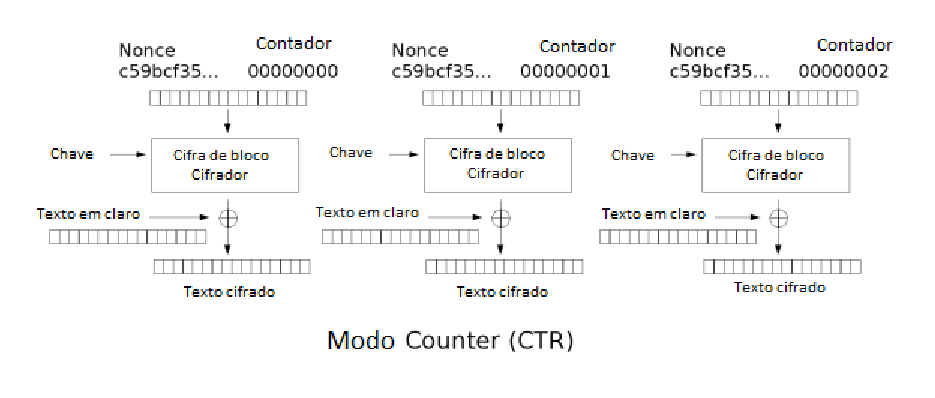
\includegraphics[keepaspectratio=true,scale=0.5]
    {figuras/ctr.eps}
    \caption{\textit{Counter Mode} } 
\end{figure}\footnote{$http://crypto.stackexchange.com/questions/8151/counter-mode-static-iv-but-different-keys$}
\end{description}

\subsection{Cifra de Fluxo}
\label{stream-cipher}

Os algoritmos que utilizam a cifra de fluxo o fazem bit a bit ou byte a byte. Uma das vantagens da cifra de fluxo em relação a cifra de bloco é seu desempenho superior e, por esse motivo, é muito utilizado em sistemas de redes,tais como \textit{bluetooth}, \textit{SSL} e outros. Outra vantagem é a possibilidade de transformar uma cifra de bloco em cifra de fluxo. Para isto basta definir que o tamanho do bloco seja bit ou byte. Alguns dos algoritmos de fluxo mais populares que, hoje cobrem mais de 80$\%$ do mundo na telecomunicação e \textit{cyber space}, são: A5/1, A5/2, E0 e RC4. ~\cite{majid-mohd}
\begin{figure}[h]
\centering
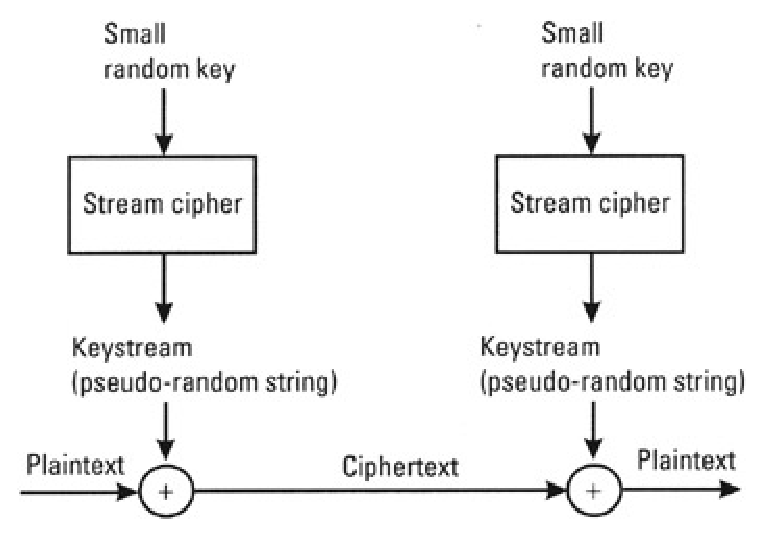
\includegraphics[keepaspectratio=true,scale=0.7]
    {figuras/stream_cipher.eps}
    \caption{\textit{Funcionamento da cifra de fluxo } } 
\end{figure}\footnote{$http://www.globalspec.com/reference/81191/203279/2-6-stream-ciphers$}

Normalmente, a cifra de fluxo utiliza 
\subsubsection{Algoritmo A5/1}
\label{algorithm-a51}

Principal algoritmo usado no mundo para a comunicação \textit{GSM}, foi desenvolvido em 1987 e teve seu funcionamento mantido em segredo e somente em 1999 foi revelado por engenharia reversa. Consiste de três \textit{Linear Feedback Shift register} ou \textit{LFSR} binários R1, R2 e R3 com cronômetro irregular. Um LFSR é um registrador que mantém valores de estado anterior e é atualizado por uma função que normalmente é um ou-exclusivo. 

Cada registrador contém bits importantes para a criptografia e que suas posições são predeterminadas. São os bit do \textit{clocking} e os \textit{tapping}. Os registradores tem tamanhos diferentes sendo que o R1 tem 19 bits, o R2 tem 22 bits e o R3 tem 23 bits. O algoritmo tem como entradas a chave secreta \textit{Kc}, que tem 64 bits e um vetor de inicialização de 22 bits composto do \textit{frame number}. O \textit{keystream}, de 228 bits, é a saída do processo, sendo que os primeiros 114 bits são o \textit{keystream} de \textit{downlink} e os outros 114 bits são o \textit{keystream} de \textit{uplink}.Cada ciclo no algoritmo é composto por passos específicos em cada registrador:

\begin{enumerate}
\item função ou-exclusivo em cada um dos \textit{tapping bits}.
\item utilizando a regra de maioridade com os \textit{clocking} bits. O registrador então é acionado se o valor do tempo for igual ao resultado da regra de maioridade então os bits do registrador é deslocado da direita para esquerda.
\item se o registrador for acionado, então o resultado do ou-exclusivo do primeiro passo deve ser passado para a posição zero do registrador correspondente.
\end{enumerate}

Finalmente com saída o ou-exclusivo do R1[18], R2[21] e R[22]. Para a fase de iniciação é utilizado a chave de 64 bits e passa de bit por bit fazendo ou-exclusivo da posição 0 de cada registrador com o bit da chave. O algoritmo ignora o resultado das primeiras 100 execuções e depois devolve os bits do \textit{keystream} a cada 228 ciclos, gerando 228 bits de saída.

\subsubsection{Algoritmo A5/2}
\label{algorithm-a52}

Esse algoritmo tem uma estrutura similar ao A5/1, com algumas exceções como por exemplo: o A5/2 utiliza 4 registradores. Outra diferença é o fato que o cronômetro dos registradores R1,R2 e R3 são acionados baseados na regra de maioridade do R4. Ou seja cada registrador é acionada dependendo dos bits do registrador R4. 

Caso o resultado seja igual ao do bit 3 então o registrador 2 é acionado, caso seja igual ao bit 7 então o registrador 3 é acionado e se for igual ao bit 10 então o registrador 1 é acionado. Depois que os registradores são acionados, então o registrador 4 é acionado também. O restante é igual ao A5/1, incluindo os 228 bits de saída do processo.
\subsubsection{Algoritmo E0}
\label{algorithm-e0}

Utilizado para proteger informações que utilizam a tecnologia \textit{bluetooth}. O principal objetivo dessa tecnologia é conectar dois aparelhos para transferência de algum tipo de informação.

O algoritmo também é baseado no uso de registradores e a saída é gerada em ou-exclusivo de bits de cada registrador. Nessa estrutura são utilizados 4 registradores com tamanhos 25, 31, 33 e 39 bits. O sistema da geração do \textit{keystream} é um pouco diferente, a cada \textit{clock tick} todos os registradores são acionados e é feito um ou-exclusivo da saída de cada um.

\subsubsection{Algoritmo RC4}
\label{algorithm-rc4}

Projetado em 1987 por Ron Rivest, é muito utilizado em sistemas de redes como TLS/SSL e WEP por conta de sua simplicidade e alto desempenho. Tem tamanho de chave variável e se baseia em permutações aleatórias.

%
\section{Criptografia Assimétrica}
\label{assymmetric-cryptography}

%
A criptografia assimétrica é usada principalmente para cifrar dados pequenos. Um dos principais usos é a assinatura digital e para realizar a troca de chaves. Esse tipo de criptografia está associada à criptografia de chave pública. Nela é estabelecido que um par de chaves (chave pública e privada) sejam usadas para a cifração e decifração da mensagem. 

%
O funcionamento é simples. Bob tem suas duas chaves e disponibiliza sua chave pública de forma que qualquer pessoa que tenha interesse em lhe enviar uma mensagem criptografada utilize sua chave pública. Quando Bob recebe a mensagem cifrada, é realizada a decifração dessa mensagem utilizando sua chave privada.

%
Alguns dos algoritmos mais conhecidos são o Elgamal e o Diffie-Hellman. O algoritmo \textit{RSA} foi o primeiro algoritmo a cifrar e decifrar com sucesso utilizando o princípio da chave pública. O Elgamal tem sua força proveniente da dificuldade de se calcular um logaritmo discreto. Com o Elgamal pode-se realizar a assinatura digital de um documento. O Diffie-Hellman foram os visionários da chave pública, primeiramente definiram a idéia e algum tempo depois definiram um algoritmo que serve apenas para trocar uma chave secreta entre duas pessoas.  Na tabela abaixo descrevemos os principais usos de cada algoritmo. 



\subsection{Algoritmo RSA}
\label{algorithm-rsa}

Tem seu nome baseado nas iniciais dos cientistas do \textit{MIT} que o inventaram: \textit{Ron Rivest, Adi Shamir} e \textit{Len Adleman}. A geração das chaves desse algoritmo é feita utilizando números primos e sua força está associada ao fato que é fácil realizar a multiplicação de dois números primos grandes, mas é difícil a decomposição desse resultado. Portanto a chave é gerada da seguinte forma:

\begin{enumerate}
\item Dois números \textbf{p} e \textbf{q} são escolhidos de forma aleatória e são primos.
\item \textbf{p} $\neq$ \textbf{q}
\item \textbf{n} é composto pela multiplicação de \textbf{p} e \textbf{q}.
\item \textbf{e}, tal que mdc($\phi$(n, e)) = 1
\item \textbf{d}, (e $^ {(-1)}$) * (mod $\phi$(n)) 
\end{enumerate}

%
A chave pública "e" é usada para criptografar a mensagem e a chave privada "d" é usada para descriptografar. O método de crifra é simples, o texto é tratado como conjunto de inteiros e a cada inteiro é feito o seguinte cálculo:

\begin{description}
\item [Criptografar]
C = M $^ e$ mod n. Sendo que M é o inteiro correspondente a parte da mensagem em claro e n o resultado da multiplicação dos dois números primos selecionados na confecção  das chaves, C é a mensagem cifrada e \textbf{e} é a chave pública. 
\item [Descriptografar]
M = C $^ d$ mod n. Sendo que C é o texto criptografado, M a mensagem em claro e \textbf{d} é a chave privada.
\end{description}

%